\section{Film Pre-characterization}\label{sec:film-pre-characterization}

\begin{figure}[htp]
  \centering
  \begin{minipage}[t]{0.48\linewidth}
    \centering
    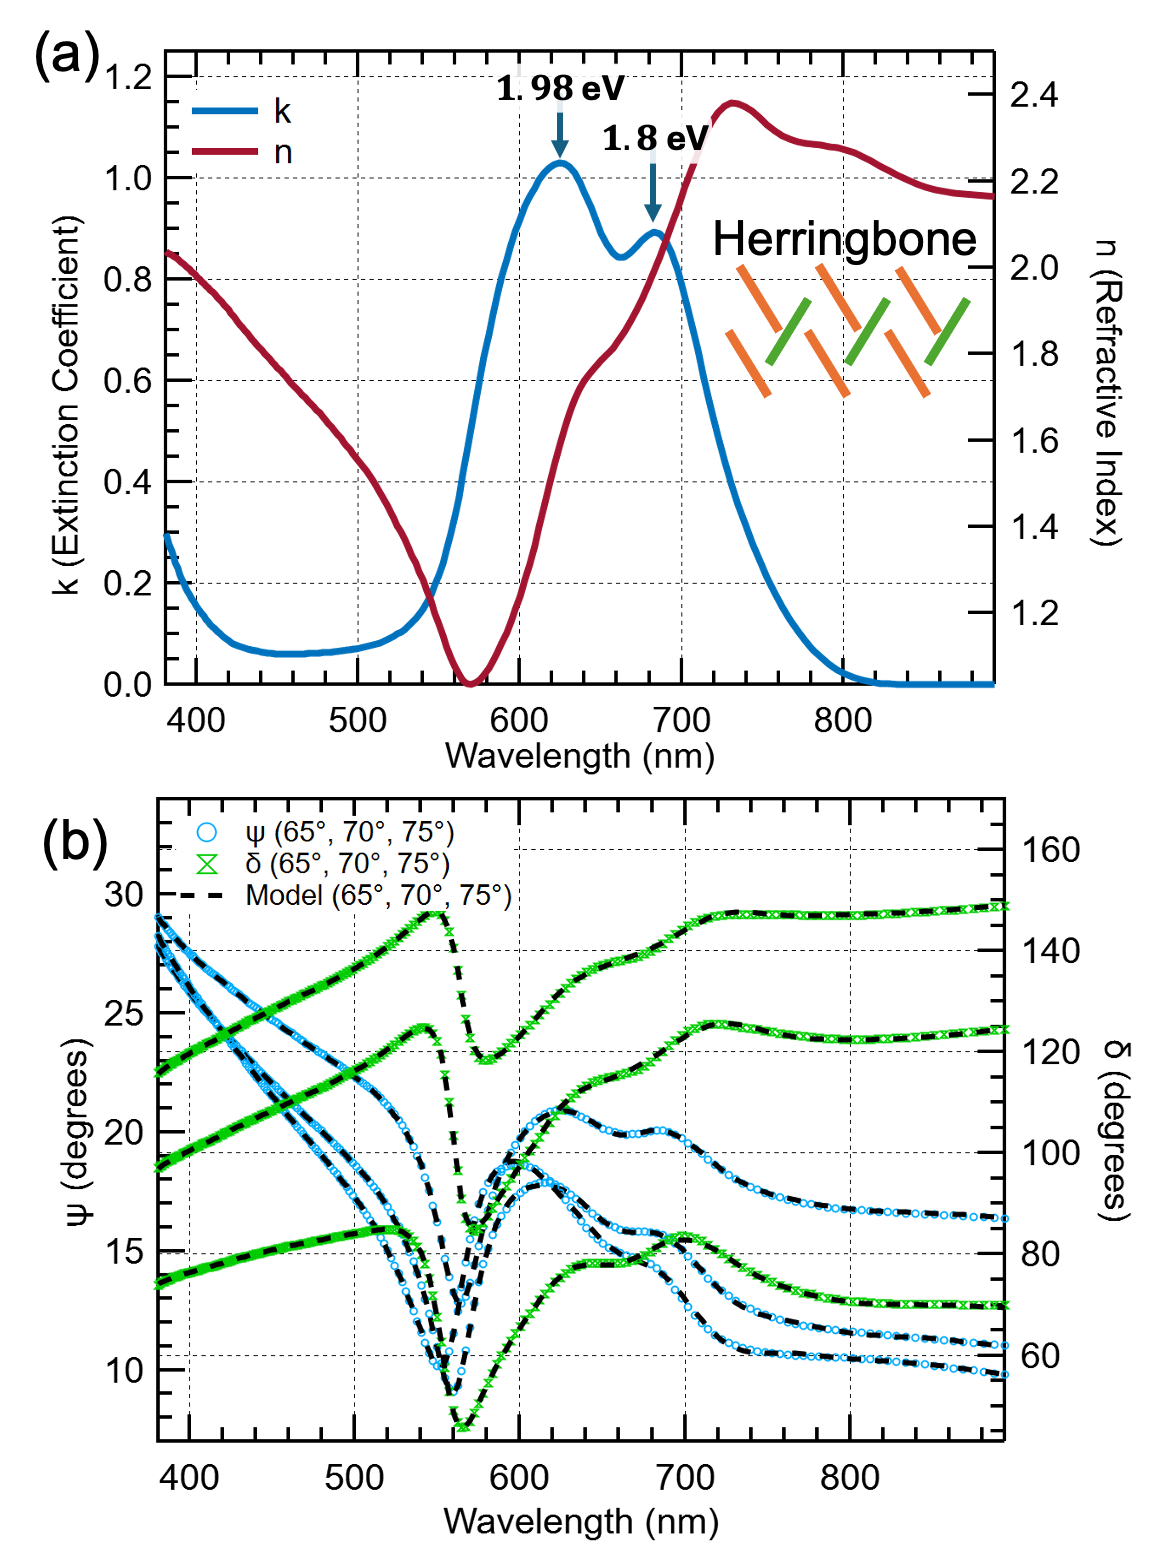
\includegraphics[width=\linewidth,height=0.6\textheight,keepaspectratio]{figS01_vase}
    \caption[VASE for ZnPc films.]{VASE for ZnPc films. (a) Optical constants derived from the VASE fit, highlighted is the Q-band splitting at \qty{625}{nm} (\qty{1.98}{eV}) and \qty{690}{nm} (\qty{1.80}{eV}) indicative of herringbone phase ZnPc packing motifs. (b) Fit results for each incidence.}
    \label{fig:S1}
  \end{minipage}\hfill
  \begin{minipage}[t]{0.48\linewidth}
    \centering
    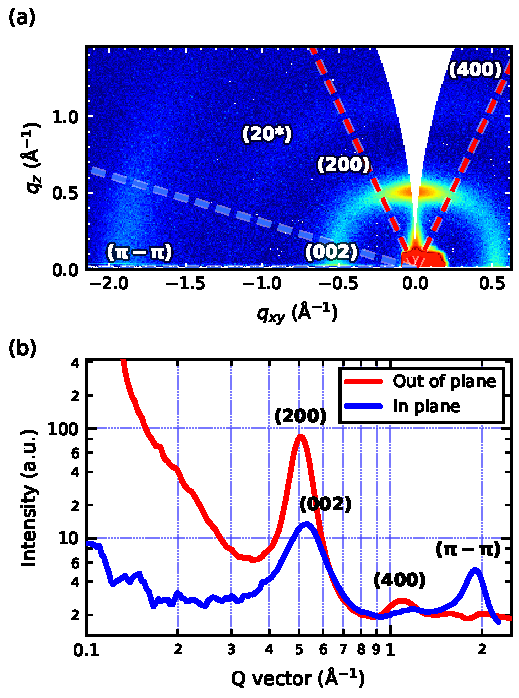
\includegraphics[width=\linewidth,height=0.6\textheight,keepaspectratio]{figS02_giwaxs}
    \caption[GIXRD for ZnPc films.]{GIXRD for ZnPc films. (a) GIWAXS image of ZnPc deposited on native-oxide silicon substrate. (b) 1D reduction showing the out-of-plane (200) peak at \qty{0.50}{\per\angstrom} (\(d\)-spacing \qty{12.6}{\angstrom}), its broadened second order (400) near \qty{1}{\per\angstrom}, the in-plane (002) peak at \qty{0.53}{\per\angstrom} (\qty{11.8}{\angstrom}) as well as a mixed index \(\pi\)-\(\pi\) stacking peak at \qty{1.89}{\per\angstrom} (\qty{3.3}{\angstrom}). Weak arcs near \(\pm\)\ang{45} from the substrate normal, markers (20*) in (a), are tentatively assigned to a mixed-index reflection but are too broad azimuthally for a definitive index.}
    \label{fig:S2}
  \end{minipage}
\end{figure}


\textbf{Variable angle spectroscopic ellipsometry}: The extinction coefficient exhibits a split Q band at 1.98 and \qty{1.80}{eV} characteristic of Davydov coupling between the translationally inequivalent molecules of the herringbone packed motif. That the higher energy peak is more intense, suggests the edge on herringbone (\(\alpha\) family) polymorph previously reported for as-deposited ZnPc in both UV-Vis and ellipsometry derived optical constants.\autocite{kozlikOpticalConstantsVZincIIPhthalocyanine2013,schunemannEvaluationControlOrientation2013} ZnPc layer thickness is recorded as \(t_{ZnPc} = 21.4(5)\) nm with a MSE of 1.433, consistent with the QCM report during deposition.

\textbf{Grazing incidence wide angle X-ray scattering:} The GIWAXS texture corroborates the polymorph and orientation assignments assigned though ellipsometric optical constants. The out-of-plane (200) reflection at \(d = \qty{12.6}{\angstrom}\) together with the in-plane (002) and \(\pi - \pi\) stacking reflections place the film in agreement with edge-on textured ZnPc on weakly interacting oxides.\autocite{derrienInterfacialRearrangementsStrain2022,schunemannEvaluationControlOrientation2013} The (200) spacing matches the relaxed \(\gamma\)-ZnPc (herringbone / \(\alpha -\)II family) value of 12.67 \(\mathring{\mathrm{A}}\) rather than the strained early growth spacing observed in the initial layers of growth.\autocite{derrienInterfacialRearrangementsStrain2022}

\begin{figure}
  \centering
  \begin{minipage}[t]{0.48\linewidth}
    \centering
    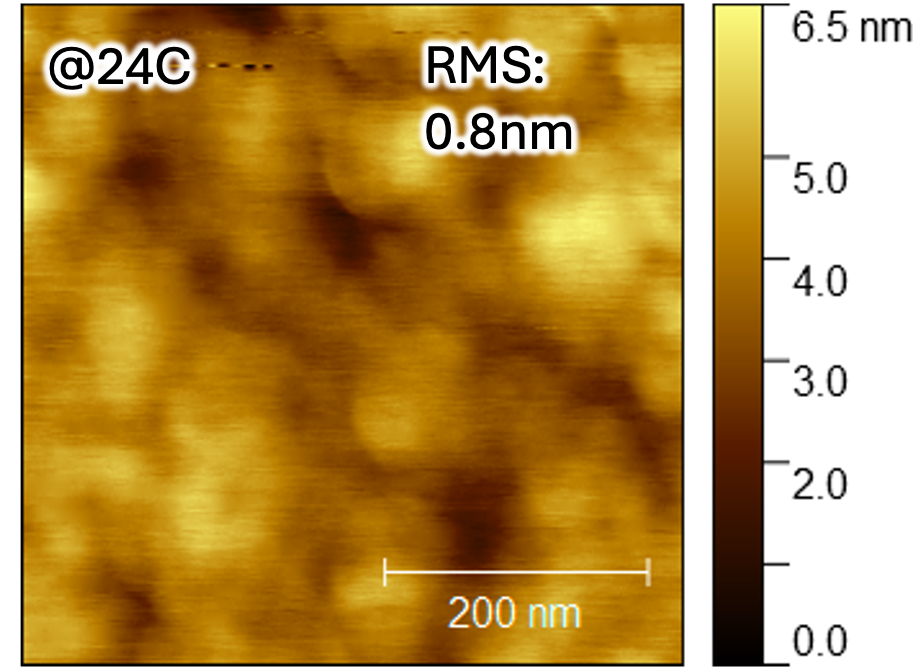
\includegraphics[width=\linewidth,height=0.6\textheight,keepaspectratio]{figS03_afm}
    \caption[AFM height map of ZnPc sample from the same batch used for RSOXS measurement.]{AFM height map of ZnPc sample from the same batch used for RSOXS measurement. RMS roughness measured as \qty{0.8}{nm}.}
    \label{fig:S3}
  \end{minipage}\hfill
  \begin{minipage}[t]{0.48\linewidth}
    \centering
    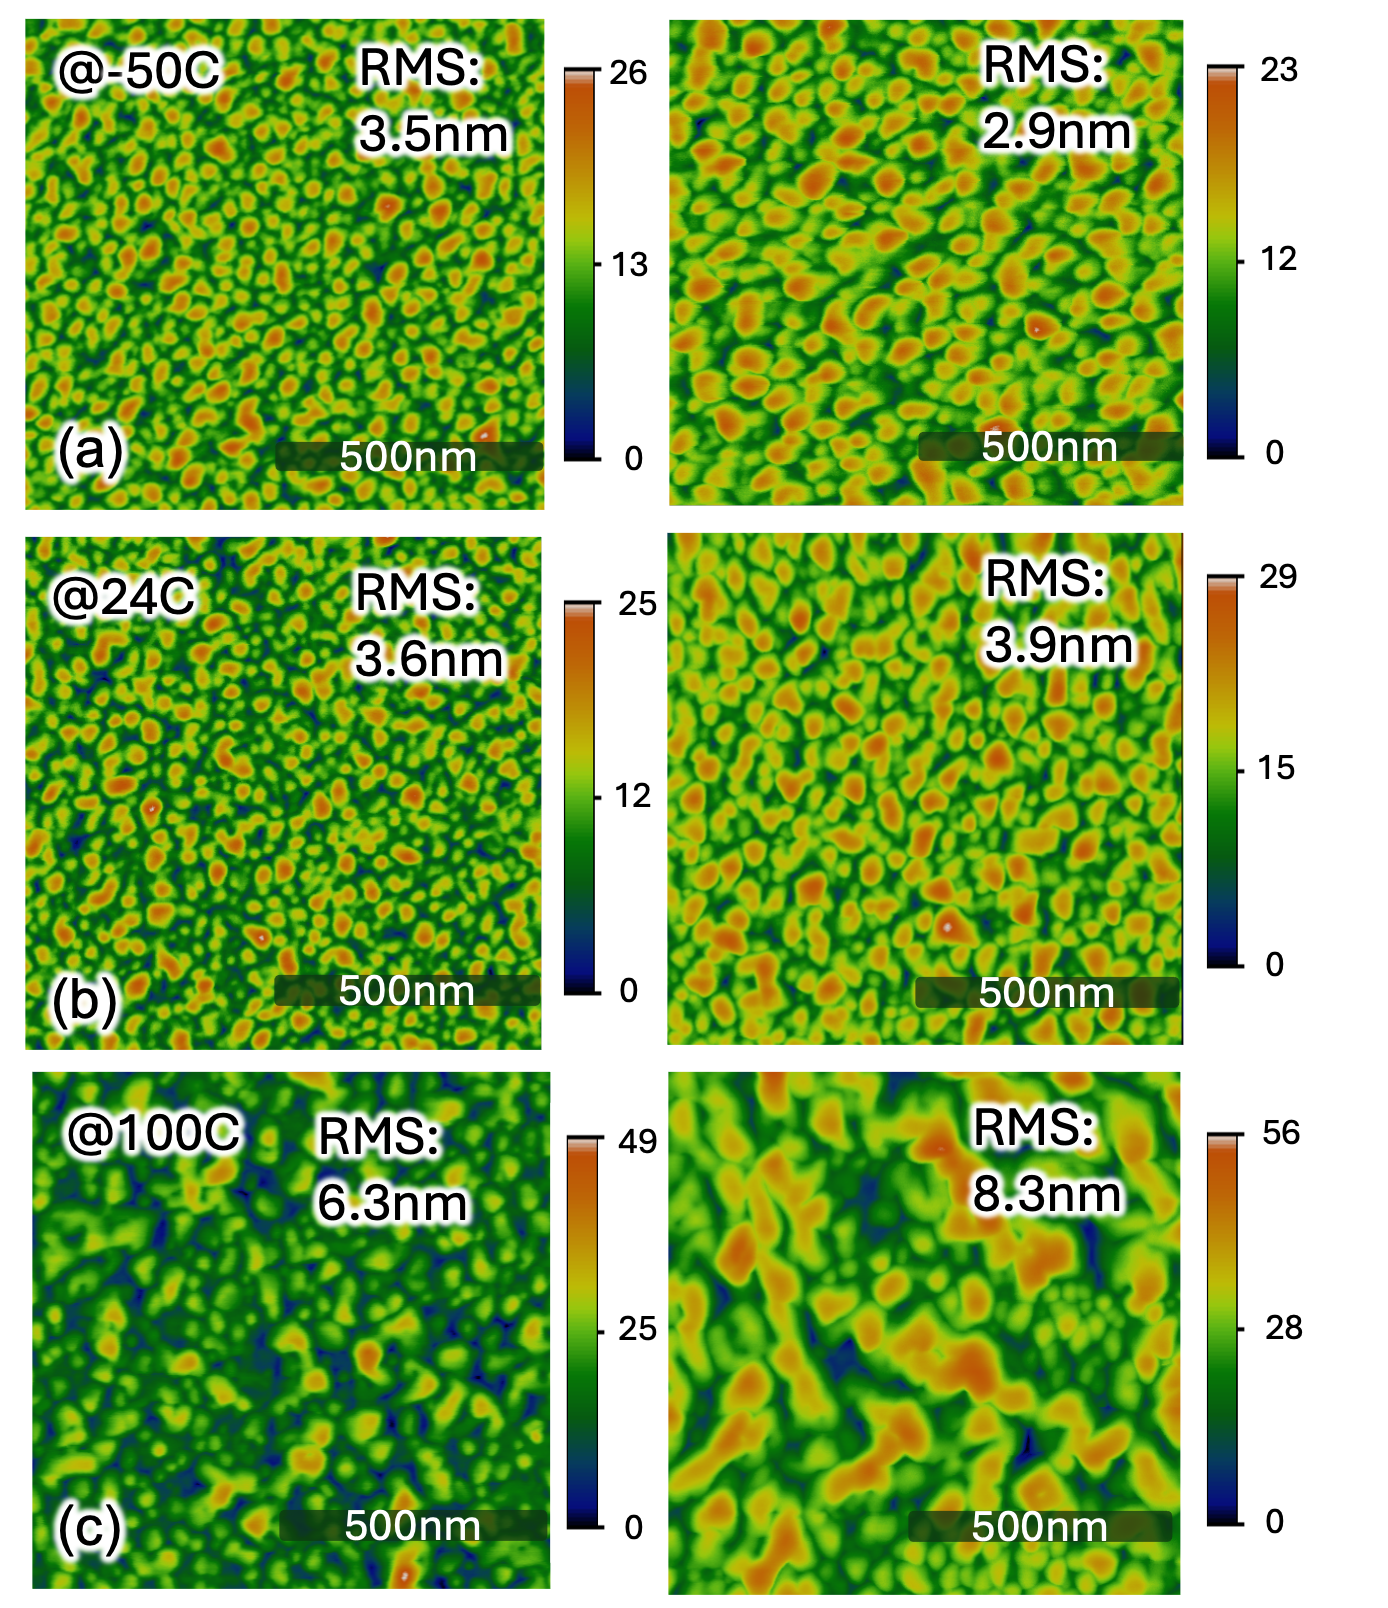
\includegraphics[width=\linewidth,height=0.6\textheight,keepaspectratio]{figS04_afm-deposition}
    \caption[AFM height map of ZnPc under different deposition conditions.]{AFM height map of ZnPc under different deposition conditions. (a-c) ZnPc deposited on a \qty{3}{nm} CuI patterning layer as a function of deposition rate (left \qty{0.15}{\angstrom\per\s}, right \qty{0.5}{\angstrom\per\s}) and substrate temperature, (a) \qty{-50}{\celsius}, (b) room temperature, \qty{24}{\celsius}, and (c) \qty{100}{\celsius}.}
    \label{fig:S4}
  \end{minipage}
\end{figure}

\textbf{Atomic force microscopy:} Atomic force microscopy (AFM) height maps were acquired on a Bruker Dimension Icon in tapping mode with a TESPA-V2 SAMPLE probe. Scans where processed using Gwyddion\autocite{necasGwyddionOpensourceSoftware2012} to extract root-mean-square (RMS) roughness values. Film morphologies and RMS roughness values were used to pre-characterize film surface roughness and morphology reflectivity measurements (\cref{fig:S3}).

\textbf{Effect or growth parameters for Copper (II) Iodide patterned films:} A film series was prepared for ZnPc grown on a \qty{3}{nm} CuI patterning layer to identify deposition conditions to make suitable RSoXS samples. Samples were grown to a target of \qty{20}{nm} as measured via QCM and validated through spectroscopic ellipsometry. AFM height maps were performed for the series and displayed below.

The surface texture for these films shows dense, laterally uniform grains with significant RMS roughness across the series. Increasing temperature leads to the formation of larger grains with more dispersity amongst their size. At 100C the morphology is most dependent on deposition rate, with the higher rate resulting in elongated domains and a larger RMS roughness. Across all conditions, film heights vary by more than the approximate layer thickness (\textgreater{} \qty{20}{nm}) suggesting that ZnPc does not form fully wetted and continuous layers when deposited on CuI, in agreement with prior work in device applications.\autocite{chikamatsuIdentifyingMolecularOrientation2018} As such we surmise that when deposited on CuI, layers grow under the Volmer-Weber (island) process, developing towers of ZnPc as opposed to continuous layer formation. Reflectivity was attempted but could not be reduced to a reliable specular dataset due to the dominant off specular signal, consistent with incomplete surface coverage

\begin{figure}
  \centering
  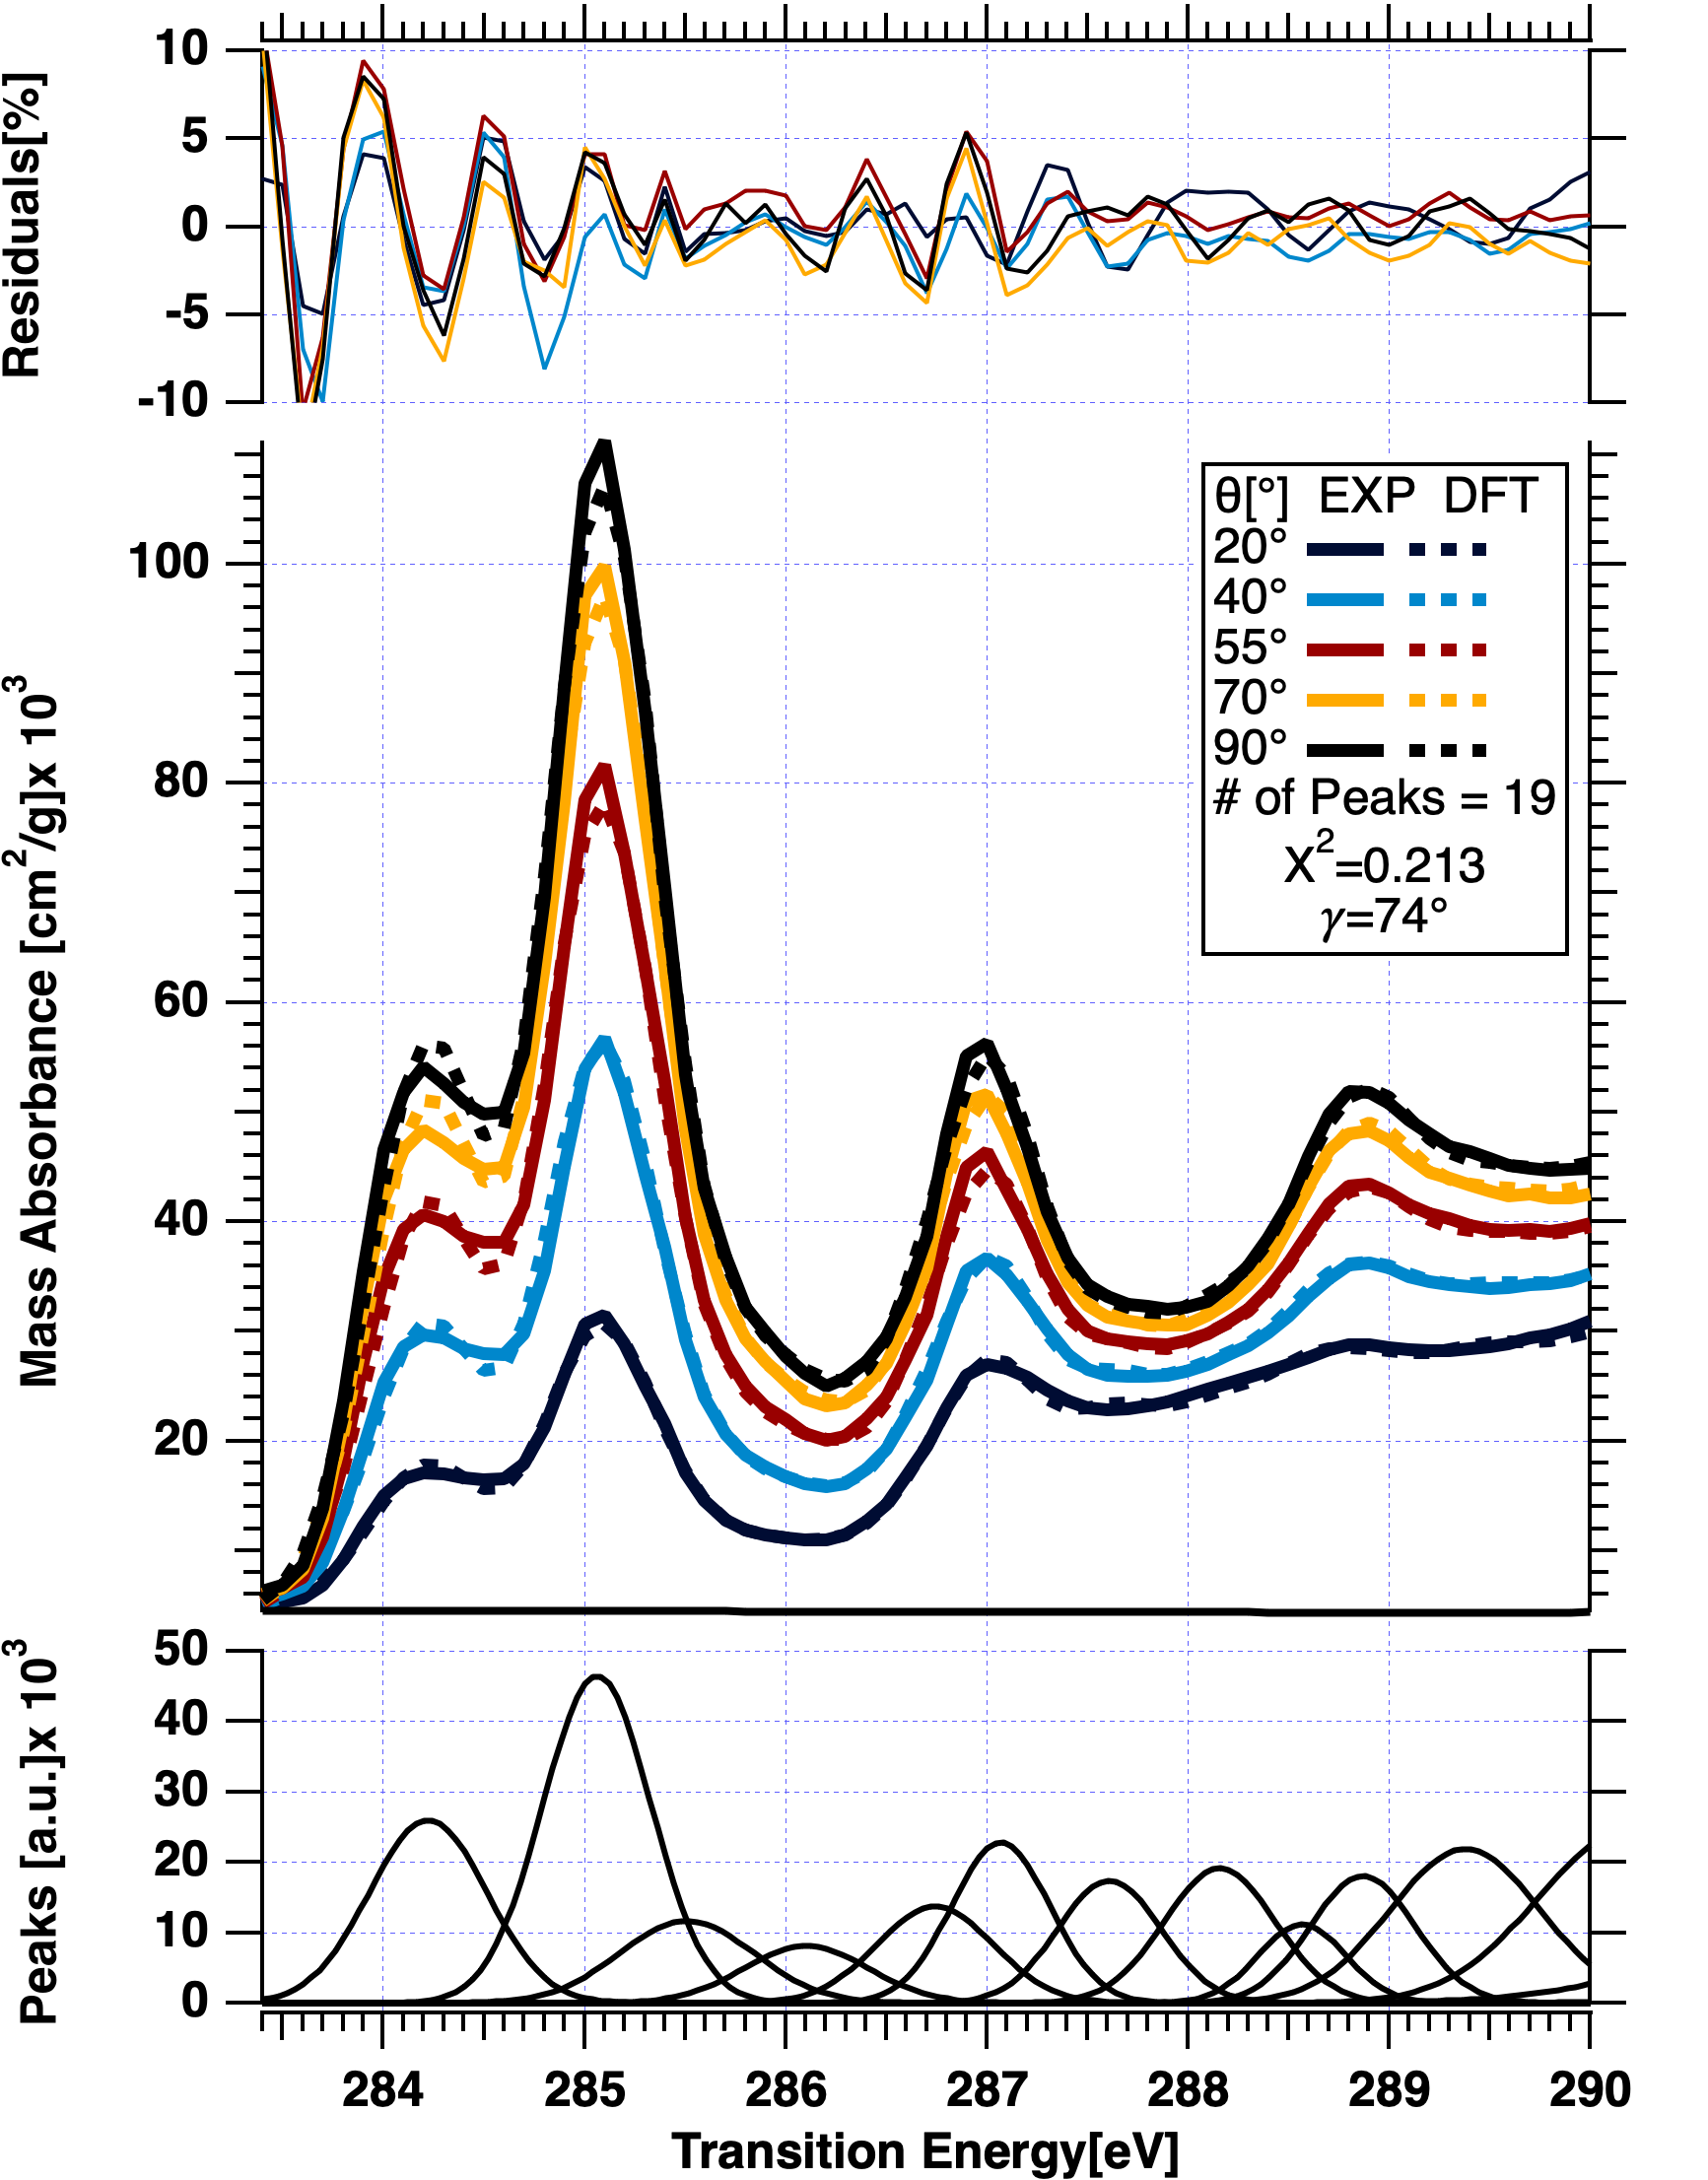
\includegraphics[width=0.45\linewidth,height=0.75\textheight,keepaspectratio]{figS05_model-comparison}
  \caption[Comparison of refined clustered optical model with experimental NEXAFS spectroscopy.]{Comparison of refined clustered optical model with experimental NEXAFS spectroscopy. The molecular tilt angle is \ang{74}, determined through the refinement of clustered DFT.}
  \label{fig:S5}
\end{figure}

\textbf{NEXAFS Spectroscopy:} NEXAFS spectroscopies were collected at the Soft X-ray Spectroscopy (SXR) beamline of the Australian Synchrotron, part of ANSTO in total electron yield mode on Si wafers. Samples were prepared under similar conditions as for RSoXS measurements yet were collected via a separate batch. Spectra were collected at five sample alignments with respect to the incident electric field polarization vector with respect to the surface normal (\(\ang{20},\ \ang{40},\ \ang{55},\ \ang{70},\ \&\ \ang{90}\)). NEXAFS was collected over the energy range of 270-\qty{350}{eV} and normalized to the energy dependent intensity fluctuation and optical loss via a direct photodiode measurement, and Au mesh drain current. Mass absorption was computed via normalization in the pre and post edge regions to the bare atom mass absorption of ZnPc as extracted from the CXRO Henke atomic scattering factors.\autocite{henkeXRayInteractionsPhotoabsorption1993}

Molecular tilt angle was extracted via the DFT cluster and refinement process. As the final step of the refinement process, the molecular polar tilt angle \(\gamma\) is fit using the TDM cluster orientations prescribed by DFT providing a measure of the molecular orientation. This fit produces a reduced \(\chi^{2}\) goodness of fit statistic of .213 indicating very good agreement between the model and experimental data. The molecular tilt angle of \(\ang{74}\) agrees with all other characterizations of the ZnPc edge-on herringbone polymorph described in this study and is taken as the coarse-grained molecular orientation within the films measured under RSoXS.

Optical Tensor Construction

The optical tensor is defined under the convention \(n(E) = 1 - \delta(E) + i\beta(E)\). From experimental NEXAFS the imaginary component is computed directly from the mass absorption spectra:

\begin{equation}
  \beta(E) = \frac{\mu\rho}{2k},
  \label{eq:S-beta}
\end{equation}

where \(\mu\) is the mass absorption, \(\rho\) is the mass density, and \(k\) the wave number.

The NEXAFS spectra is scaled to agree with the bare atom mass absorption as tabulated by the CXRO with a density of one.\autocite{CXROXRayInteractions} This constructs an index of refraction specific volume that we use to evaluate the index of refraction for a given material density. The real part of the refractive index \(\delta(E)\) is computed via the Kramers-Kronig calculation using the KKcalc package.\autocite{wattsCalculationKramersKronigTransform2014}

The experimental tensor components are constructed following the established empirical method.\autocite{ferronCompositionDictatesMolecular2023,collinsPolarizedXrayScattering2012} From clustering, the primary \(\pi^{*}\) TDM cluster rests at \({.01}^{\circ}\) from the molecular normal. The NEXAFS derived dichroism across the carbon edge is computed by taking the average difference spectra between all pairs of incident angles as a function of energy. This constructs an experimental dichroism that is used to augment the isotropic \(\beta_{iso}(E)\) measured at the magic angle to recover the refractive tensor components from the molecular reference frame, i.e.,

\begin{align}
  \beta_{zz}(E) &= \beta_{\mathrm{iso}}(E) + A(\theta)\Delta\beta(E), \label{eq:S-beta-zz}\\
  \beta_{xx}(E) &= \beta_{\mathrm{iso}}(E) - B(\theta)\Delta\beta(E), \label{eq:S-beta-xx}
\end{align}

The coefficients \(A(\theta)\) and \(B(\theta)\) are defined to match the condition in Stöhr, modified to accommodate the off axis TDM polar angle \(\theta\) associated with the primary transition.

\begin{align}
  A(\theta) &= \left( 3\cos^{2}\theta - 1 \right)\frac{\beta_{\mathrm{iso}}(E_{\pi})}{\Delta\beta(E_{\pi})}, \label{eq:S-A}\\
  B(\theta) &= \frac{\tfrac{1}{2}\left( 3\cos^{2}\theta - 1 \right)\beta_{\mathrm{iso}}(E_{\pi})}{\Delta\beta(E_{\pi})}. \label{eq:S-B}
\end{align}

The DFT tensor is instead defined using the directly calculated tensor components for each TDM cluster, resulting in the comparison of Fig.~4.1, requiring no auxiliary analyses.

\section{DFT Methods}\label{sec:dft-methods}

\begin{figure}[htp]
  \centering
  \begin{minipage}[t]{0.48\linewidth}
    \centering
    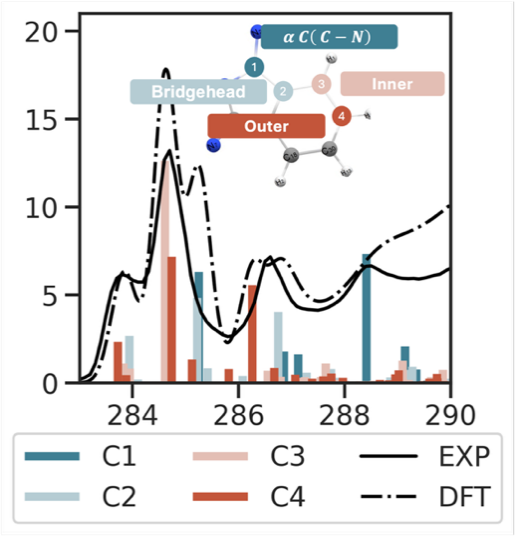
\includegraphics[width=\linewidth,height=0.6\textheight,keepaspectratio]{word-export/figS6}
    \caption[DFT calculated NEXAFS spectroscopy for ZnPc computed from the four highlighted excitation centers vs transition energy, overlapped with experimental NEXAFS from the SXR beamline.]{DFT calculated NEXAFS spectroscopy for ZnPc computed from the four highlighted excitation centers vs transition energy, overlapped with experimental NEXAFS from the SXR beamline. Poles indicate individual contributing oscillators.}
    \label{fig:S6}
  \end{minipage}\hfill
  \begin{minipage}[t]{0.48\linewidth}
    \centering
    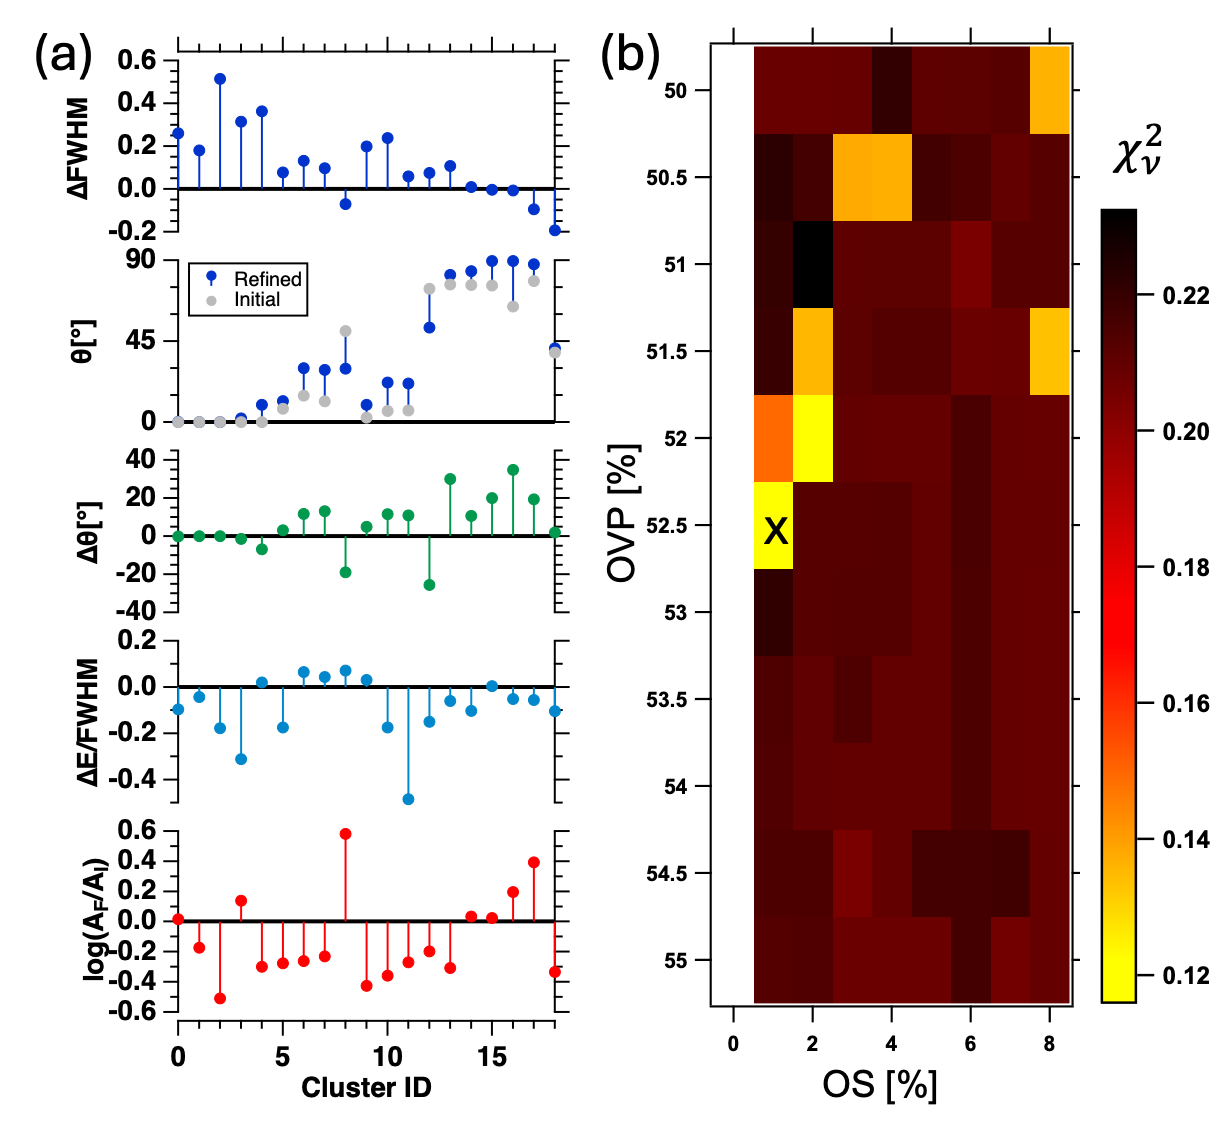
\includegraphics[width=\linewidth,height=0.6\textheight,keepaspectratio]{figS07_clustering}
    \caption[Clustering and refinement analysis.]{Clustering and refinement analysis. (a) Change in parameters though the refinement process for the chosen set of hyperparameters. (b) OVP \% and OS \% hyperparameter optimization map}
    \label{fig:S7}
  \end{minipage}
\end{figure}


A time independent transition potential calculation using the StoBe library was performed on a single molecule of ZnPc. A HCH approach sets the manifold of transition energies, along with each TDM and oscillator strength, while the \(\Delta KS\ \)method is used to fix the absolute energy associated with each transition. For details see our previous work.\autocite{murciaQuantitativeBondTraceableResonant2026} The molecular geometry was extracted from a crystallographic structure file (.cif) as it produced results with a higher initial agreement to experiment compared to thermodynamically relaxed structures, or those relaxed from molecular force fields.

From this structure, four chemically distinct carbon atoms (labeled in Fig.~4.1 and \cref{fig:S6}) set the primary excitation centers for the molecule. Calculations using the eight carbons of the entire outer molecular wing, along with the 16 for half of the molecule, were tried yet offered no improved accuracy and only increased dimensionality and complexity of the calculation results. Here we demonstrate that a reduced set of excitation reproduces the entire set of transitions possible for molecular ZnPc, and though clustering provides an optical model that is useful for scattering analysis.

\textbf{Clustering and Refinement:} Clustering and refinement were performed using the Igor Pro implementation of the hierarchical agglomerative clustering to extract a set of TDM clusters as the initial building blocks for the optical model. Oscillator strength threshold and Overlap percentage hyperparameters were explored using an evenly spaced support via

\begin{equation*}
  \mathrm{OS} \in [0, 10], \qquad \mathrm{OVP} \in [25, 75]
\end{equation*}

Hyperparameter pairs were evaluated by reduced chi square to experimental NEXAFS and well-behaved parameter pairs where secondarily evaluated by their difference form the original DFT, ensuring the preservation of the DFT calculated information. Here we chose the best fit clustering parameters of \(OS = .25\) and \(OVP = 52.5\). In general, we find good clustering and convergence for all \(OVP \in \lbrack 50,55\rbrack\), with significantly worse performance outside of these bounds. Moreover, we find that \(OS \in \lbrack.1,8\rbrack\) performed similarly, yet parameter agreement with originating DFT degrades rapid for larger \(OS\), while the refinement never converse for \(OS < .1\).

\section{Optical Model Parameterization}\label{sec:optical-model-parameterization}

Molecular order within the film is parameterized by the molecular tilt angle \(\gamma\) of the molecular surface normal from the film surface normal. For uniaxial film, this is the polar cone angle. We begin with the single molecule refined DFT optical model. This construction assumes the single molecule DFT is representative of the electronic states available to a film of the material, ignoring the creation of new multi molecule states, that could be caused by variations to molecular packing or orientation alignment. However, as the clustered DFT model agrees with the experimentally derived optical model, we surmise that these effects are not dominant in this system.

We start with the uniaxial molecular optical tensor\({\ n}^{m}\) constructed through clustering,

\begin{equation}
  n^{m}(E) = \begin{pmatrix} n_{xx} & 0 & 0 \\ 0 & n_{xx} & 0 \\ 0 & 0 & n_{zz} \end{pmatrix},
  \label{eq:S-molecular-tensor}
\end{equation}

where \(n_{xx}\) is the in plane or ordinary component, and \(n_{zz}\) is the out of plane or extraordinary component. The molecule is then tilted by an arbitrary polar angle \(\gamma\) about the \(x\) or \(y\)-axis, the choice being arbitrary, before computing the uniform azimuthal average over \(\phi \in \lbrack 0,2\pi\rbrack\), i.e.,

\begin{equation}
  n^{f}(E,\gamma) = \left\langle R^{\mathsf{T}}(\phi,\gamma)\, n^{m}(E)\, R(\phi,\gamma) \right\rangle_{\phi}.
  \label{eq:S-film-average}
\end{equation}

where \(\phi\) is the dummy azimuthal orientation variable, and \(R(\phi,\gamma)\) the product \(R_{z}(\phi)R_{x/y}(\gamma)\). Because the material and refined molecular tensor are azimuthally symmetric, the off diagonal components vanish by inspection and, with a density scale factor, the ZnPc optical tensor reduces to,

\begin{align}
  n_{xx}^{f}(E;\gamma,\rho) &= \frac{\rho}{2}\left[ n_{xx}^{m}\left( 1 + \cos^{2}\gamma \right) + n_{zz}^{m}\sin^{2}\gamma \right], \label{eq:S-film-xx}\\
  n_{zz}^{f}(E;\gamma,\rho) &= \rho\left( n_{xx}^{m}\sin^{2}\gamma + n_{zz}^{m}\cos^{2}\gamma \right). \label{eq:S-film-zz}
\end{align}

To validate these results, we find the isotropic condition is \(\gamma = \arcsin\sqrt{2/3} \approx \ang{54.7}\) the so-called magic angle, in agreement with Stöhr.\autocite{stohrNEXAFSSpectroscopy1992}

\section{RSoXS Experimental and Analysis Methods}\label{sec:rsoxs-experimental-and-analysis-methods}

\textbf{RSoXS Collection:} RSoXS measurements were performed at advanced light source beamline 11.0.1.2 following the standard procedures established by Ferron et. al. Using the scatter slits and higher order suppressor optical elements, the direct beam intensity was attenuated to a reasonable level for direct measurement on the photodiode detector. In this configuration, the beam was aligned using the in-chamber photodiode detector via the following. A knife edge experiment is used to align the sample z-motor position. Then from this z position, the sample theta motor is offset to 1-2 degrees. The detector theta motor is then scanned over a 4-degree window around the corresponding 2theta position. By recursively performing sample-z-and-theta alignment scans the sample can be aligned to the center of the goniometer axis of rotation to within .01 deg. Note that motor issues, beam drift, and tilt along the sample plate, the axis alignment must be recalibrated during extended runs, especially after changing polarization or substantially changing beamline energy.

Experimental data was collected starting in the s-pol configuration, beginning at \qty{250}{eV} and working to the resonant energies realigning the axis of rotation after every 10 energies. Between polarizations, the alignment was recalibrated after waiting for 30 min for the new heat load to affect the optics. Measurements were performed over a 12-hour shift with an energy calibration performed using the transmission NEXAFS of polystyrene, at the start and end of the shift showing no energy drift throughout the experiment duration.

\textbf{Reflectivity Reduction}: Reflectivity measurements are reduced from 2D images by first locating the specular reflected beam on the area detector and integrating the intensity within a suitable region. A background signal is removed from this intensity using a region of the detector far from the specular beam spot. This background region is collected along the same row as the beam spot to account for systematic CCD readout noise. The measured reflectance is then computed from the specular reflected intensity by dividing by the incident \(I_{0}\) intensity collected at the start of each energy scan.

High dynamic range sensitivity was achieved by slicing the measurement q-range into subsets with overlapping points where the reflected intensity could be well captured on the two orders of magnitude of dynamic range allotted by the CCD detector. This is done by using the higher order suppressor optical element and increasing the exposure time. Using the overlapping points, an effective \(I_{0}\) intensity can be determined for each subset used in the calculation of reflectance for long q-range scans.

\textbf{Error Approximations:} Each frame of a reflectivity profile is inherently a photon counting measurement. The raw intensity in each detector pixel follows a poissonian distribution to first approximation, giving a per-pixel error equal to \(\sqrt{N}\). Systematic noise is also present, originating from the dark current, readout noise, and stray light. Readout noise is reduced by first trimming a 10-pixel border around the images and then performing a row-by-row subtraction using the average counts from the first 10 pixels in every row of the detector image. This flattens the thermal background caused by the readout process. The stray light and dark current can then be modeled and accounted for using the dark region of the detector as described above. Non-poissonian noise is characterized using a Fano factor defined as the ratio of the observed variance in \(I_{0}\) and effective \(I_{0}\) measurements to the hypothesized poissonian variance at the same intensity level. This effectively scales the raw poissonian noise in each q subset.

The final source of error comes in the discrimination between specular and off specular reflectance. Thin film surface scattering and roughness effects smear the reflected beam over a finite width of pixels. This effect becomes more pronounced at higher q-values. To account for this error a q-dependent uncertainty envelope is applied to the propagated uncertainties from data reductions producing a higher uncertainty in the higher q regions of spectra.

\textbf{RSoXS Analysis Methods:} Our fitting methodology has been largely updated from the procedures outlined in Ferron et. al.\autocite{ferronCompositionDictatesMolecular2023} The model was constructed containing three layers of ZnPc (Surface, Bulk, Interface), on top of a thin SiO\textsubscript{2} native oxide layer, followed by the Si substrate. Each ZnPc layer is modeled using a uniaxial optical tensor whose derivation is described in the methods above. The reflection and transmission coefficients for the stack are computed for each energy and scattering vector via the 4x4 transfer matrix formalism where boundary condition matching at each of the five interfaces sets the reflection and transmission coefficients for each layer, while interfacial roughness manifests as anexponential attenuation to account for the off specular diffuse scattering from a faceted interface. Here we model interfacial roughness in the Nèvot-Croce (NC) sense as is standard for reflectivity analyses.\autocite{nevotCaracterisationSurfacesPar1980,esashiInfluenceSurfaceInterface2021} This sets the parameterization of the physical model structure as thickness and roughness for the surface, bulk, and interface layers of ZnPc, along the native SiO\textsubscript{2} layer for a combined eight parameters to set the full structure.

\begin{figure}
  \centering
  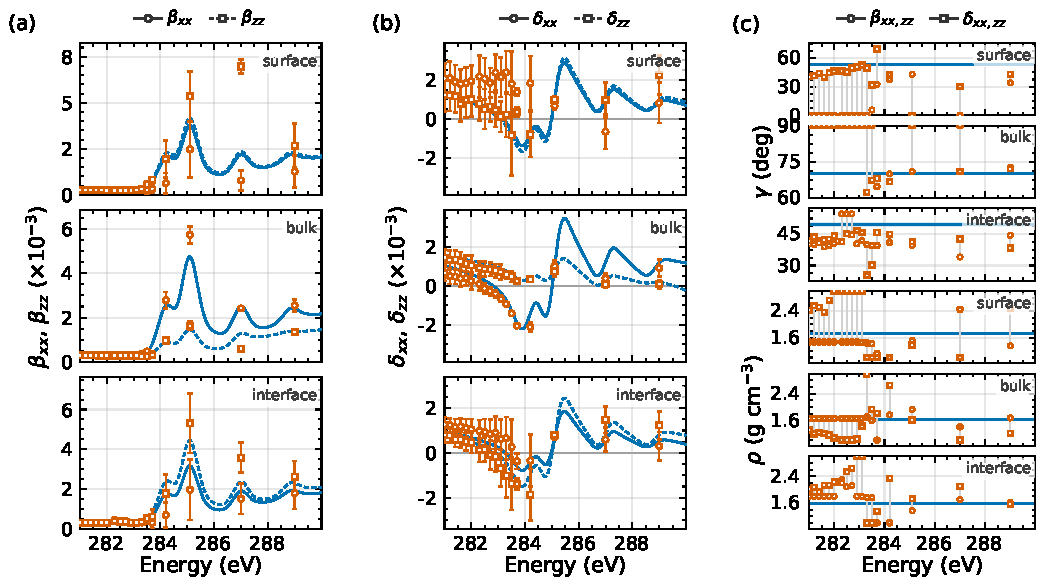
\includegraphics[width=\linewidth,height=0.75\textheight,keepaspectratio]{figS08_optical-constants}
  \caption[Comparison in final best fit optical constants revealed through the Free optical tensor and DFT models.]{Comparison in final best fit optical constants revealed through the Free optical tensor and DFT models. (a) Imaginary tensor components β, (b) real tensor components δ. The extracted orientation and density are compared in (c) and (d) where the directly refined orientation from the DFT model (traces) is compared with the per energy orientation computed from a secondary refinement to the full tensor. The density is determined by the magnitude of the trace of the optical tensor and showcases a much lower inter energy variance. The orientation that sets dichroism and birefringence varies much strongly between energies and amongst q-ranges.}
  \label{fig:S8}
\end{figure}

The optical constants for each layer are set depending on the optical model and differ between the free tensor and DFT parameterization. Consistent across both are the non-resonant material slabs for the vacuum and silicon fronting media, along with the silicon dioxide layer. Each are set with tabulated bare atom optical constants, parameterized by the energy independent material density that we allow to vary subtly from the tabulated values to accommodate differences in stoichiometry, but fixed to a feasible region of (2, 2.8) g/cm\textsuperscript{3}. The optics for free tensor ZnPc are parameterized as birefringence, dichroism, isotropic \(\delta_{iso}\), and isotropic \(\beta_{iso}\) each constrained to a reasonable range dictated by the original optical model and following the choices by Ferron et. al. resulting in 252 optical tensor components for the present work. The DFT optics are set energy independently via a molecular orientation and density per layer, along with an energy offset term common across all layers and accounting for the energy calibration differences between instruments resulting in just seven parameters to describe the three ZnPc layers. Thus, the free tensor parameterization uses 266 (8+2+252) parameters to describe the material, while the DFT model uses just 17 (8+2+7) to describe the same structure, over an order of magnitude in reduced complexity.

The free tensor parameterization is the most general model and differs from the best analyses by Ferron et. al.\autocite{ferronCompositionDictatesMolecular2023} In prior works, a dichroic ratio is used to set the ratio between the birefringence and dichroism for the material allowing for a reduction of one degree of freedom per energy in the model. However, correctly computing this requires the creation of the energy dependent optical tensor wile resulting in only a 3/4 reduction in optical parameters still requiring the fitting of the birefringence per energy. This fails to enforce cross energy consistency checks such as the Kramers-Kronig relations or the consistency in molecular orientation between energies. As a result, in our comparisons, we take the full tensor complexity for our Free tensor model.

The reflectivity model calculating reflectivity from the material stack is augmented to include several experimental correction terms that account for beam and motor drifts, along with instrument miscalibration during the measurement. This includes a normalization correction scale factor and an angle of incidence offset applied to each energy and polarization, following the analysis of Ferron et. al.\autocite{ferronCompositionDictatesMolecular2023} Combined this adds in four correction terms per energy (84 in this work) accounting for a majority of the fitted parameters in our DFT constrained optical model. This brings the total model parameters to 101 for the DFT model and 350 for the Free tensor model.

For those seeking to follow this analysis, experimental correction parameters can often be critical to producing a good fit. However, it is important to note that without proper bounds on a per energy basis, experiment correction parameters easily become cross-correlated with both the structure and optics leading to non-physical fit results. We recommend only adding these offset parameters if the first fringe is challenging to reproduce using physically realistic structural and optical parameters. Reasonable bounds on the normalization correction term are (.8, 1.2) with exceptions for datasets with visible outliers in the \(I_{0}\) measurement points. Angle of incidence may vary more widely from zero, and manual observations of the data should be used to set a feasibility region of this parameter. Here we use bounds of (-.1, .1) due to the measurable alignment drift across energies. Additionally, as ALS 11.0.1.2 and other future RSoXS capable instruments constantly improve their configurations, these ranges should be discussed with the beamline scientist for the instrument for the latest insights.

\textbf{Fit Results:}

\begin{figure}
  \centering
  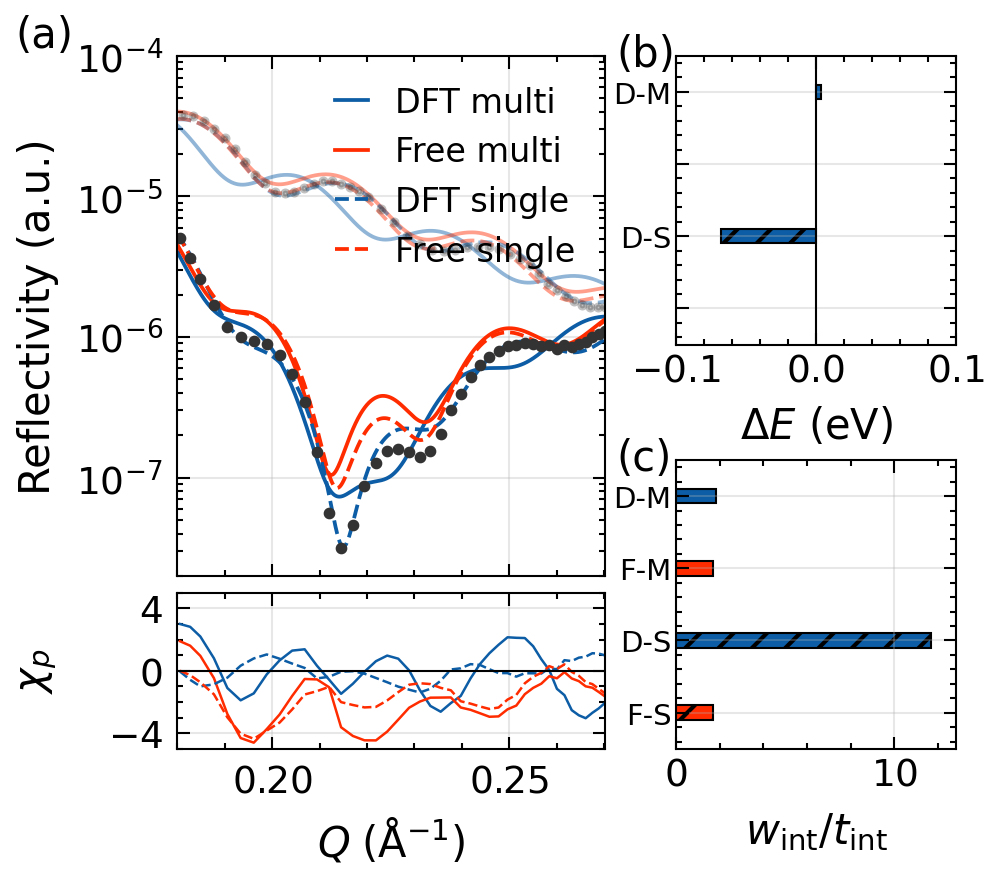
\includegraphics[width=0.45\linewidth,height=0.75\textheight,keepaspectratio]{figS09_single-energy-fits}
  \caption[Comparison of single energy reflectivity fits at the diagnostic energy (\qty{283.7}{eV}) against the multi energy refinement.]{Comparison of single energy reflectivity fits at the diagnostic energy (\qty{283.7}{eV}) against the multi energy refinement. (a) Direct fit comparison and residuals showcasing that the DFT single energy can out-perform other fit strategies within Brewster’s angle. (b) Energy offset parameter results used in the fits compared between the DFT multi energy (D-M) and single energy (D-S) fits indicating that the single energy fit must take an extreme \qty{-0.1}{eV} offset, to a non-absorbing energy. (c) Interfacial width \(w = 2\pi\sigma_{r}\) of the interface layer showcasing that the D-S fit is more than \(10\times\) the total thickness of this buried layer.}
  \label{fig:S9}
\end{figure}

\begin{table}
  \centering
  \caption{Best fit structural properties of the ZnPc film extracted using the Free tensor optical model. Errors are reported as \(2\sigma\) from the covariance matrix.}\label{tab:S1}
  \begin{tabular}{l S[table-format=3.2(2)] S[table-format=2.2(2)]}
    \toprule
    Layer & {\(t\) (\unit{\angstrom})} & {\(\sigma_{r}\) (\unit{\angstrom})} \\
    \midrule
    Surface & 8.8(4) & 7.21(28) \\
    Bulk & 174.4(4) & 10.43(31) \\
    Interface & 14.48(24) & 8.39(15) \\
    \bottomrule
  \end{tabular}
\end{table}

\begin{table}
  \centering
  \caption{Best fit structural properties of the ZnPc extracted using the ML-DFT slab optical model. Errors are reported as \(2\sigma\) from the covariance matrix.}\label{tab:S2}
  \begin{tabular}{l S[table-format=3.3(1)] S[table-format=2.3(1)] S[table-format=2.2(1)] S[table-format=1.3(1)]}
    \toprule
    Layer & {\(t\) (\unit{\angstrom})} & {\(\sigma_{r}\) (\unit{\angstrom})} & {\(\gamma\) (\unit{\degree})} & {\(\rho\) (\unit{g.cm^{-3}})} \\
    \midrule
    Surface & 8.933(4) & 7.056(1) & 52.21(7) & 1.8(3) \\
    Bulk & 179.95(3) & 13.136(2) & 69.54(1) & 1.638(3) \\
    Interface & 10.705(2) & 7.892(5) & 47.24(9) & 1.0(6) \\
    \bottomrule
  \end{tabular}
\end{table}

\section{Orientation Gradient Theoretical Foundation}\label{sec:orientation-gradient-theoretical-foundation-1}

We formulate our gradient model from a Ginzburg-Landau framework of second order phase transitions, where we treat the molecular orientation and density as order parameters (not to be confused with nematic order parameters \(S(\gamma)\) or \(P(\gamma)\)).\autocite{gennesPhysicsLiquidCrystals2023,Ginzburg2009} Along the one dimensional depth axis \(z\) of a film of thickness \(L\), we take the order parameters as the deviation in the density \(\Delta\rho(z) = \rho(z) - \rho_{b}\) and orientation \(\Delta\gamma(z) = \gamma(z) - \gamma_{b}(z)\) from the bulk. The total free energy of the film is described by the functional

\begin{equation}
  \begin{split}
  F[\Delta\rho,\Delta\gamma] &= \int_{0}^{L} \left[ f(\Delta\rho,\Delta\gamma) + \frac{1}{2}c_{\rho}\left( \Delta\rho' \right)^{2} + \frac{1}{2}c_{\gamma}\left( \Delta\gamma' \right)^{2} \right] dz \\
  &\quad + F_{v}\left[ \Delta\rho(0),\Delta\gamma(0) \right] + F_{\mathrm{Si}}\left[ \Delta\rho(L),\Delta\gamma(L) \right].
  \end{split}
  \label{eq:S-free-energy}
\end{equation}

Here \(f(\Delta\rho,\Delta\gamma)\) is the local bulk free energy density, and the terms proportional to \(c_{\rho}\) and \(c_{\gamma}\) are the gradient energy penalties that oppose abrupt variations within the film. The interface terms \(F_{v}\) and \(F_{Si}\) account for the anchoring potentials at the interface boundaries. Expanding \(f(\Delta\rho,\Delta\gamma)\) to quadratic order about the bulk minimum,

\begin{equation}
  f(\Delta\rho,\Delta\gamma) \approx f_{0} + \frac{1}{2}a_{\gamma}\Delta\gamma^{2} + \frac{1}{2}a_{\rho}\Delta\rho^{2} + b\,\Delta\rho\,\Delta\gamma,
  \label{eq:S-local-free-energy}
\end{equation}

where \(a_{\rho}\) and \(a_{\gamma}\) are the stability coefficients of the bulk phase, and \(b\) the bilinear coupling term between the density and orientation fields.

Minimizing the total variation \(\delta F = 0\) and integrating the gradient terms by parts yields a system of coupled second-order differential equations for the film interior,

\begin{align}
  c_{\rho}\,\Delta\rho'' &= a_{\rho}\Delta\rho + b\,\Delta\gamma, \label{eq:S-el-rho}\\
  c_{\gamma}\,\Delta\gamma'' &= a_{\gamma}\Delta\gamma + b\,\Delta\rho, \label{eq:S-el-gamma}
\end{align}

with boundaries dictated by the surface free energies. To leading order in the interface fields \(h\), the boundary variation yields Robin boundary conditions, where the gradient of the order parameter is proportional to the surface field, i.e.

\begin{equation}
  c_{\rho}\Delta\rho'(0) = - h_{\rho}^{v}, \qquad c_{\rho}\Delta\rho'(L) = h_{\rho}^{\mathrm{Si}},
  \label{eq:S-robin}
\end{equation}

and with similar form for \(\Delta\gamma\). In the limit of strong anchoring, the surface fields \(h\) are much stronger than the bulk stiffness coefficients \(c/\tau\), the system enters the Dirichlet regime. Here each interface potentials set the order parameters to fixed interfacial values, \(\Delta\rho(0) = {\Delta\rho}_{v}\) and \(\Delta\rho(L) = {\Delta\rho}_{Si}\). Within this regime the interfaces impose an orientational state regardless of the bulk interaction, a feasible state given the known different growth modes for ZnPc films at the substrate and surface.\autocite{derrienInterfacialRearrangementsStrain2022,yangMolecularOrientationInducedRapidRoughening2015}

This system of equations may be decoupled into a normal modes problem, under the coordinate transform \(\widetilde{\Delta\rho} = \sqrt{c_{\rho}}\Delta\rho\) and similar transform for \(\Delta\gamma\). Given that the bulk represents the stable minimum, the general solution is restricted to the linear combination of exponentials decaying from the boundaries with coherence lengths \(\tau_{\pm}\) derived from the eigenvalues of the coupled system. When the orientation and density coupling is nonzero, these coherence lengths are shared between the order parameters. As each interface bears its unique interactions that dictate this coherence length, we assume that each interface is dominated by a single mode. The interface gradient model used in the main text satisfies these conditions,

\begin{align}
  \Delta\rho(z) &= \Delta\rho_{v}\exp\left( - z/\tau_{\mathrm{vac}} \right) + \Delta\rho_{\mathrm{Si}}\exp\left( - (L - z)/\tau_{\mathrm{Si}} \right), \label{eq:S-profile-rho}\\
  \Delta\gamma(z) &= \Delta\gamma_{v}\exp\left( - z/\tau_{\mathrm{vac}} \right) + \Delta\gamma_{\mathrm{Si}}\exp\left( - (L - z)/\tau_{\mathrm{Si}} \right). \label{eq:S-profile-gamma}
\end{align}

While this model is congruent with the continuous reorientation under an evolving growth front, it remains an empirical approximation of the underlying interfacial physics. A more rigorous determination of the anchoring potentials would require a detailed investigation of the boundary conditions, specifically whether the system is governed by Dirichlet or Robin boundaries as this determines the relationship between exponential amplitudes and the interfacial potentials. Furthermore, this model assumes a continuous structural relaxation; however, it is possible that the molecular realignment across the interface occurs under a different mechanism than described here requiring a different theoretical basis.

\begin{figure}
  \centering
  \begin{minipage}[t]{0.48\linewidth}
    \centering
    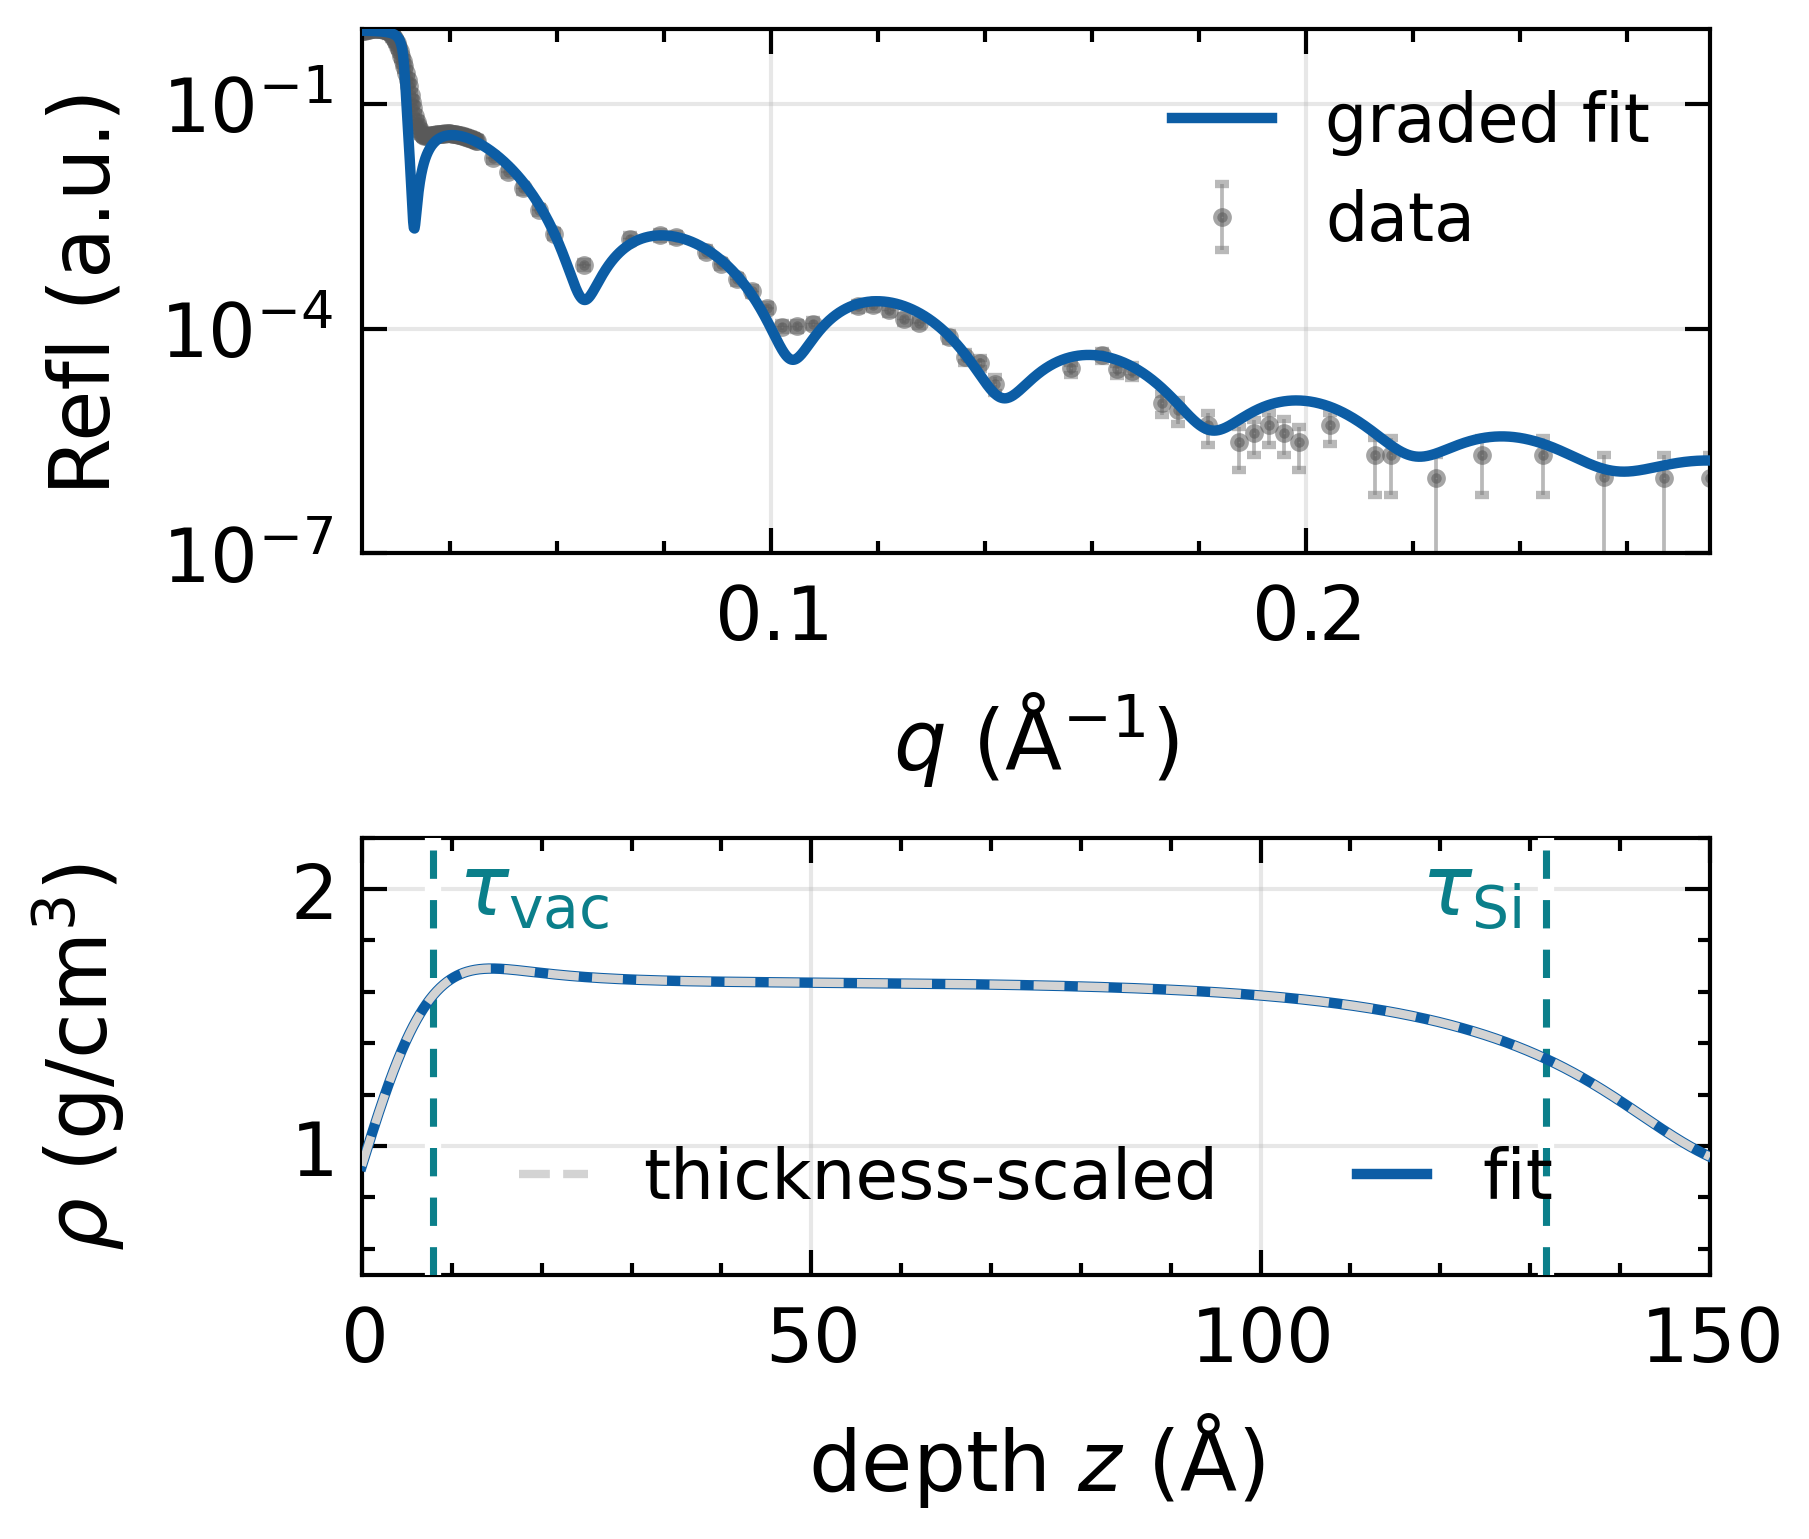
\includegraphics[width=\linewidth,height=0.6\textheight,keepaspectratio]{figS10_nonresonant-xrr}
    \caption[Non-resonant and non-polarized XRR measured on a similarly prepared sample with thickness \qty{15}{nm} measured by QCM and grown under otherwise identical conditions.]{Non-resonant and non-polarized XRR measured on a similarly prepared sample with thickness \qty{15}{nm} measured by QCM and grown under otherwise identical conditions. Data was measured at Washington State University on a Xenocs Xeuss 3.0 with a focused Cu X-ray source. Reflectivity was fit using the starting parameters of the gradient model Table~4.1 while fitting only total film thickness. Once converged all other parameters where refined, \(\rho_{v}\), \(\rho_{b}\), \(\rho_{\mathrm{Si}}\), \(\tau_{v}\), \(\tau_{\mathrm{Si}}\), to less than \(1\sigma\) from their initial position. A single non resonant energy is incapable of independently determining the orientation gradient, yet the density gradient is consistent with this second sample.}
    \label{fig:S10}
  \end{minipage}\hfill
  \begin{minipage}[t]{0.48\linewidth}
    \centering
    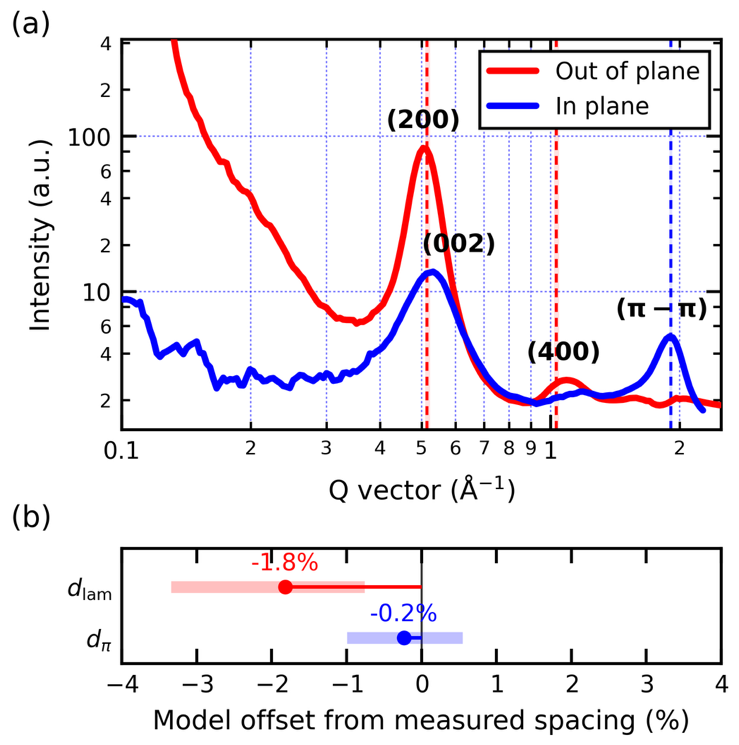
\includegraphics[width=\linewidth,height=0.6\textheight,keepaspectratio]{word-export/figS11}
    \caption[Reconstructed packing (Fig.~4.4c) compared with GIWAXS.]{Reconstructed packing (Fig.~4.4c) compared with GIWAXS. (a) Out-of-plane (red) and in-plane (blue) sector cuts from \cref{fig:S2} with lamellar orders and the π-stacking reflection indexed. Dashed lines mark the d-spacing predicted by the packing in Fig.~4.4c. (b) Comparison between predicted d-spacing and the measured d-spacing for both periods.}
    \label{fig:S11}
  \end{minipage}
\end{figure}

\begin{table}
  \centering
  \caption{Unit cell parameters for the crystal phases used in MD simulations. Literature \(\beta\)-ZnPc unit cell parameters presented and rounded for comparison.\autocite{maiDataDensityFunction2020} GIXRD constrained unit cell (EXP) compared with the (MD) relaxed cell, with uncertainties set by 10ps block averages over the final 50 ps of the simulation. Atomic coordinates for constructed \(\alpha\) cells are provided as CIFs.}\label{tab:S3}
  \begin{tabular}{l S[table-format=2.3(1)] S[table-format=1.3(1)] S[table-format=2.3(2)] S[table-format=3.3(1)] S[table-format=1.3]}
    \toprule
    Phase & {\(a\) (\unit{\angstrom})} & {\(b\) (\unit{\angstrom})} & {\(c\) (\unit{\angstrom})} & {\(\beta\) (\unit{\degree})} & {\(\rho\) (\unit{g.cm^{-3}})} \\
    \midrule
    \(\beta\) & 14.5 & 4.9 & 17.2 & 106.201(2) & 1.648 \\
    \(\alpha\) (experiment) & 24.93 & 4.18 & 23.62 & 90.4 & 1.558 \\
    \(\alpha\) (MD) & 24.647(3) & 3.917(2) & 23.985(10) & 90 & 1.657 \\
    \bottomrule
  \end{tabular}
\end{table}

\begin{figure}
  \centering
  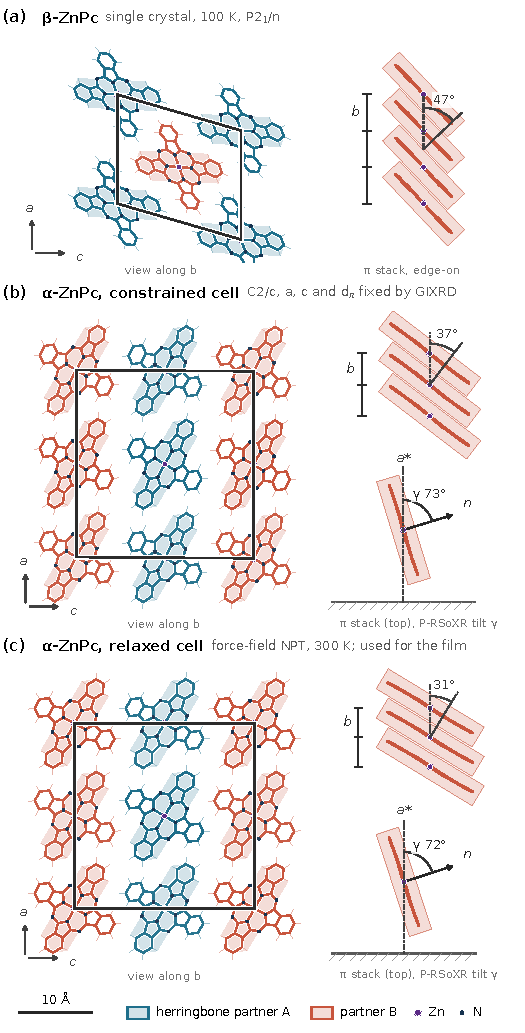
\includegraphics[width=0.55\linewidth,height=0.75\textheight,keepaspectratio]{figS12_unit-cells}
  \caption[Constructed unit cells for MD simulations.]{Constructed unit cells for MD simulations. (a) β phase ZnPc from the crystallography used for DFT simulation. (c) α phase ZnPc constructed from CuPc α cell, with spacings constrained from GIXRD. (d) Thermally relaxed α-ZnPc cell through LAMMPS simulation. The α-ZnPc cell is constructed on a repulsive wall and annealed at \qty{300}{K}.}
  \label{fig:S12}
\end{figure}

\begin{figure}
  \centering
  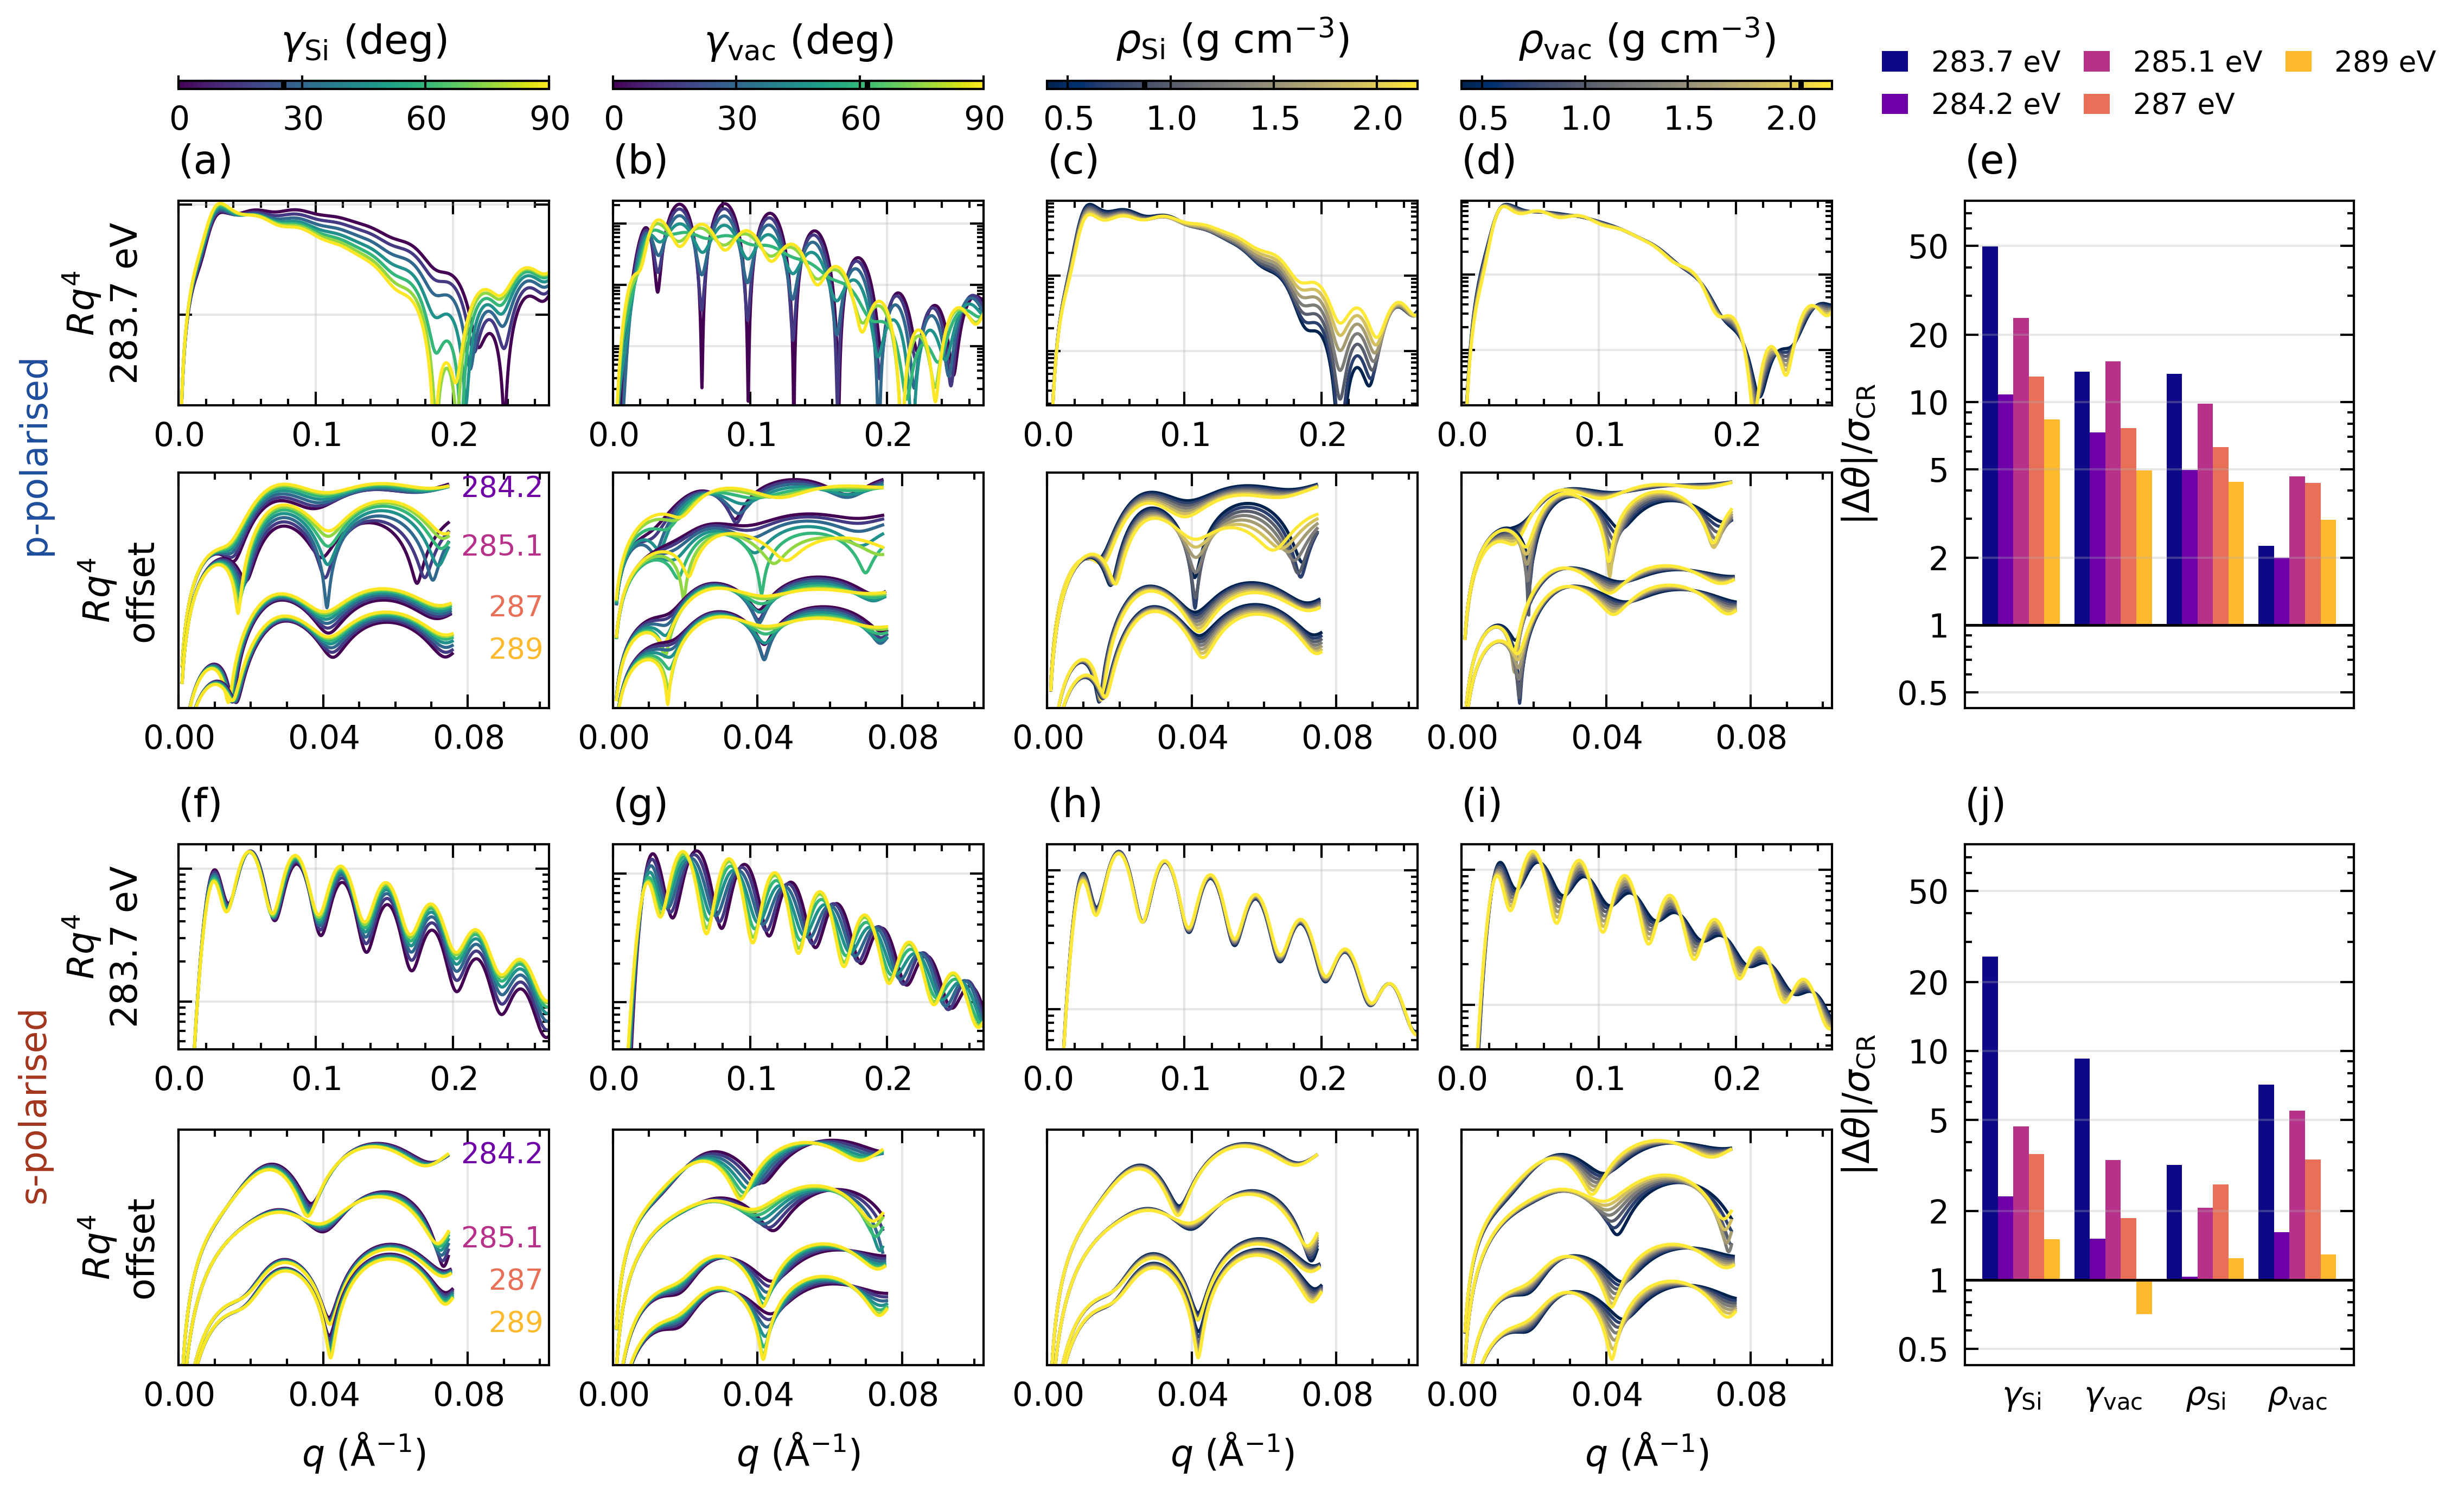
\includegraphics[width=\linewidth,height=0.75\textheight,keepaspectratio]{figS13_fisher-sensitivity}
  \caption[Fisher sensitivity analysis for reflectivity of 2nd order orientation and density phase transitions for ZnPc.]{Fisher sensitivity analysis for reflectivity of 2nd order orientation and density phase transitions for ZnPc. From the best fit model (Fig.~4.4a), each pinned boundary is systematically varied along a feasible grid with characteristic thicknesses held constant. (a-d) p-polarized and (f-i) s-polarized simulated reflectivity (\(Rq^{4}\)). The upper axis of each reflectivity panel originates from the \qty{283.7}{eV} diagnostic energy over the full measurement range, with the lower being the resonant series on the reduced q-range vertically offset for clarity. The reflectivity slope and fringe depth, that usually set by surface or interfacial roughness, are polarization and energy dependent. Moreover, the primary channel for sensitivity to the buried interface is the p-polarized reflectivity, especially for q values near Brewster’s angle causing \qty{283.7}{eV} to dominantly dictate the buried microstructure. The Kiessig fringe phase is also set differently across energy and polarization by a combination by all four pinned interfaces with no single parameter fully setting the phase. (e \& j) Detectability, \(\Delta\theta/\sigma_{\mathrm{CR}}\), for each dataset split by energy, parameter and polarization, where \(\Delta\theta\) is the difference in each parameter from the bulk phase, and \(\sigma_{\mathrm{CR}}\) is the Cramér-Rao bound. The Fisher information is evaluated at the measured q-points over every parameter of the joint fit along with the four boundary values, with the other parameters held constant. The measurement error is modified with a fractional error floor setting \(\chi^{2}_{\nu} \to 1\) such that the best fit solution in the main text is treated as the ground truth. Bars rise from one standard error, \(\Delta\theta/\sigma_{\mathrm{CR}} = 1\). The pinned silica state rises 37 and 9 standard errors from the bulk using a residual based sandwich covariance (\(\sigma_{\gamma,\mathrm{Si}} = \ang{1.28}\), \(\sigma_{\rho,\mathrm{Si}} = \qty{0.084}{g.cm^{-3}}\)).}
  \label{fig:S13}
\end{figure}
